\documentclass{standalone}
\usepackage{tikz}
\usetikzlibrary{patterns, positioning}


\begin{document}
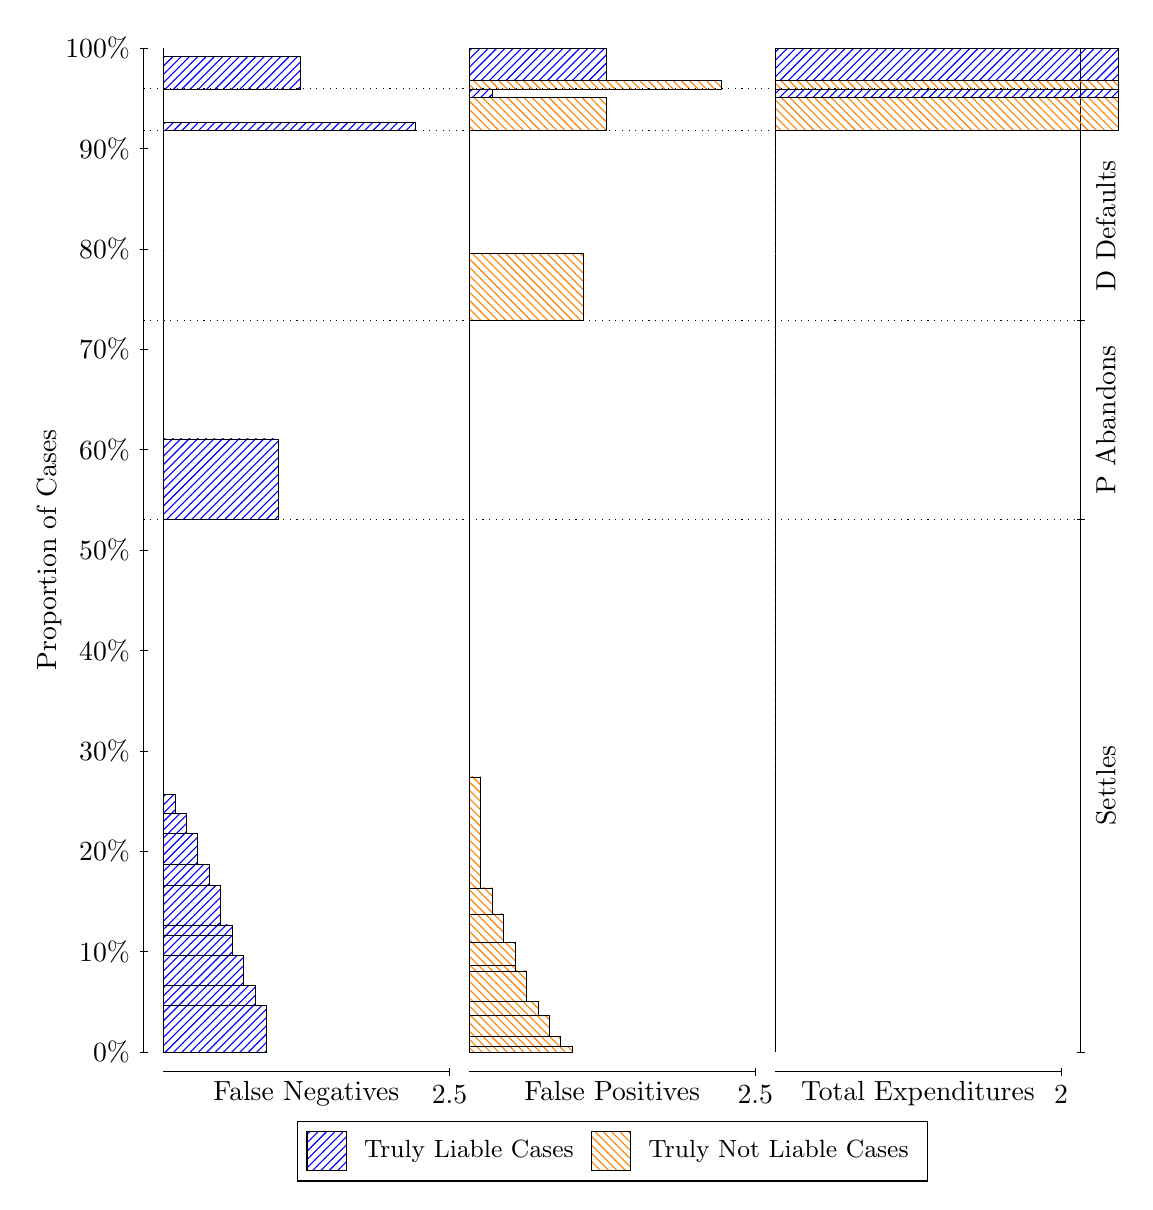
\begin{tikzpicture}
\draw[black, very thin] (1.5,1.75) -- (1.5,14.5);
\node[rotate=90, text=black, anchor=center] at (0.3, 8.125) {Proportion of Cases};
\draw[black, very thin] (1.45,1.75) -- (1.55,1.75);
\node[text=black, anchor=east] at (1.45, 1.75) {0\%};
\draw[black, very thin] (1.45,3.025) -- (1.55,3.025);
\node[text=black, anchor=east] at (1.45, 3.025) {10\%};
\draw[black, very thin] (1.45,4.3) -- (1.55,4.3);
\node[text=black, anchor=east] at (1.45, 4.3) {20\%};
\draw[black, very thin] (1.45,5.575) -- (1.55,5.575);
\node[text=black, anchor=east] at (1.45, 5.575) {30\%};
\draw[black, very thin] (1.45,6.85) -- (1.55,6.85);
\node[text=black, anchor=east] at (1.45, 6.85) {40\%};
\draw[black, very thin] (1.45,8.125) -- (1.55,8.125);
\node[text=black, anchor=east] at (1.45, 8.125) {50\%};
\draw[black, very thin] (1.45,9.4) -- (1.55,9.4);
\node[text=black, anchor=east] at (1.45, 9.4) {60\%};
\draw[black, very thin] (1.45,10.675) -- (1.55,10.675);
\node[text=black, anchor=east] at (1.45, 10.675) {70\%};
\draw[black, very thin] (1.45,11.95) -- (1.55,11.95);
\node[text=black, anchor=east] at (1.45, 11.95) {80\%};
\draw[black, very thin] (1.45,13.225) -- (1.55,13.225);
\node[text=black, anchor=east] at (1.45, 13.225) {90\%};
\draw[black, very thin] (1.45,14.5) -- (1.55,14.5);
\node[text=black, anchor=east] at (1.45, 14.5) {100\%};

\draw[black, very thin] (13.4,1.75) -- (13.4,14.5);
\draw[black, very thin] (13.35,1.75) -- (13.45,1.75);
\node[anchor=west] at (13.35, 1.75) {};
\draw[black, very thin] (13.35,8.5162) -- (13.45,8.5162);
\node[anchor=west] at (13.35, 8.5162) {};
\draw[black, very thin] (13.35,11.038) -- (13.45,11.038);
\node[anchor=west] at (13.35, 11.038) {};
\draw[black, very thin] (13.35,13.451) -- (13.45,13.451);
\node[anchor=west] at (13.35, 13.451) {};
\draw[black, very thin] (13.35,13.982) -- (13.45,13.982);
\node[anchor=west] at (13.35, 13.982) {};
\draw[black, very thin] (13.35,14.5) -- (13.45,14.5);
\node[anchor=west] at (13.35, 14.5) {};

\draw[black, very thin, pattern color=blue, pattern=north east lines] (1.75,1.75) rectangle (3.058,2.3462);
\draw[black, very thin, pattern color=blue, pattern=north east lines] (1.75,2.3462) rectangle (2.9127,2.5929);
\draw[black, very thin, pattern color=blue, pattern=north east lines] (1.75,2.5929) rectangle (2.7673,2.9753);
\draw[black, very thin, pattern color=blue, pattern=north east lines] (1.75,2.9753) rectangle (2.622,3.2345);
\draw[black, very thin, pattern color=blue, pattern=north east lines] (1.75,3.2345) rectangle (2.622,3.3636);
\draw[black, very thin, pattern color=blue, pattern=north east lines] (1.75,3.3636) rectangle (2.4767,3.8688);
\draw[black, very thin, pattern color=blue, pattern=north east lines] (1.75,3.8688) rectangle (2.3313,4.1297);
\draw[black, very thin, pattern color=blue, pattern=north east lines] (1.75,4.1297) rectangle (2.186,4.5304);
\draw[black, very thin, pattern color=blue, pattern=north east lines] (1.75,4.5304) rectangle (2.0407,4.7767);
\draw[black, very thin, pattern color=blue, pattern=north east lines] (1.75,4.7767) rectangle (1.8953,5.0222);
\draw[black, very thin, pattern color=orange, pattern=north west lines] (1.75,5.0222) rectangle (1.75,8.5162);
\draw[black, very thin, pattern color=blue, pattern=north east lines] (1.75,8.5162) rectangle (3.2033,9.5369);
\draw[black, very thin, pattern color=orange, pattern=north west lines] (1.75,9.5369) rectangle (1.75,11.038);
\draw[black, very thin, pattern color=orange, pattern=north west lines] (1.75,11.038) rectangle (1.75,11.888);
\draw[black, very thin, pattern color=blue, pattern=north east lines] (1.75,11.888) rectangle (1.75,13.451);
\draw[black, very thin, pattern color=blue, pattern=north east lines] (1.75,13.451) rectangle (4.9473,13.56);
\draw[black, very thin, pattern color=orange, pattern=north west lines] (1.75,13.56) rectangle (1.75,13.982);
\draw[black, very thin, pattern color=blue, pattern=north east lines] (1.75,13.982) rectangle (3.494,14.391);
\draw[black, very thin, pattern color=orange, pattern=north west lines] (1.75,14.391) rectangle (1.75,14.5);
\draw[black, very thin, pattern color=orange, pattern=north west lines] (5.6333,1.75) rectangle (6.9413,1.8239);
\draw[black, very thin, pattern color=orange, pattern=north west lines] (5.6333,1.8239) rectangle (6.796,1.951);
\draw[black, very thin, pattern color=orange, pattern=north west lines] (5.6333,1.951) rectangle (6.6507,2.2178);
\draw[black, very thin, pattern color=orange, pattern=north west lines] (5.6333,2.2178) rectangle (6.5053,2.3931);
\draw[black, very thin, pattern color=orange, pattern=north west lines] (5.6333,2.3931) rectangle (6.36,2.7798);
\draw[black, very thin, pattern color=orange, pattern=north west lines] (5.6333,2.7798) rectangle (6.2147,2.8492);
\draw[black, very thin, pattern color=orange, pattern=north west lines] (5.6333,2.8492) rectangle (6.2147,3.1436);
\draw[black, very thin, pattern color=orange, pattern=north west lines] (5.6333,3.1436) rectangle (6.0693,3.5023);
\draw[black, very thin, pattern color=orange, pattern=north west lines] (5.6333,3.5023) rectangle (5.924,3.8332);
\draw[black, very thin, pattern color=orange, pattern=north west lines] (5.6333,3.8332) rectangle (5.7787,5.244);
\draw[black, very thin, pattern color=blue, pattern=north east lines] (5.6333,5.244) rectangle (5.6333,8.5162);
\draw[black, very thin, pattern color=orange, pattern=north west lines] (5.6333,8.5162) rectangle (5.6333,10.017);
\draw[black, very thin, pattern color=blue, pattern=north east lines] (5.6333,10.017) rectangle (5.6333,11.038);
\draw[black, very thin, pattern color=orange, pattern=north west lines] (5.6333,11.038) rectangle (7.0867,11.888);
\draw[black, very thin, pattern color=blue, pattern=north east lines] (5.6333,11.888) rectangle (5.6333,13.451);
\draw[black, very thin, pattern color=orange, pattern=north west lines] (5.6333,13.451) rectangle (7.3773,13.873);
\draw[black, very thin, pattern color=blue, pattern=north east lines] (5.6333,13.873) rectangle (5.924,13.982);
\draw[black, very thin, pattern color=orange, pattern=north west lines] (5.6333,13.982) rectangle (8.8307,14.091);
\draw[black, very thin, pattern color=blue, pattern=north east lines] (5.6333,14.091) rectangle (7.3773,14.5);
\draw[black, very thin, pattern color=orange, pattern=north west lines] (9.5167,1.75) rectangle (9.5167,5.244);
\draw[black, very thin, pattern color=blue, pattern=north east lines] (9.5167,5.244) rectangle (9.5167,8.5162);
\draw[black, very thin, pattern color=orange, pattern=north west lines] (9.5167,8.5162) rectangle (9.5167,10.017);
\draw[black, very thin, pattern color=blue, pattern=north east lines] (9.5167,10.017) rectangle (9.5167,11.038);
\draw[black, very thin, pattern color=orange, pattern=north west lines] (9.5167,11.038) rectangle (9.5167,11.888);
\draw[black, very thin, pattern color=blue, pattern=north east lines] (9.5167,11.888) rectangle (9.5167,13.451);
\draw[black, very thin, pattern color=orange, pattern=north west lines] (9.5167,13.451) rectangle (13.877,13.873);
\draw[black, very thin, pattern color=blue, pattern=north east lines] (9.5167,13.873) rectangle (13.877,13.982);
\draw[black, very thin, pattern color=orange, pattern=north west lines] (9.5167,13.982) rectangle (13.877,14.091);
\draw[black, very thin, pattern color=blue, pattern=north east lines] (9.5167,14.091) rectangle (13.877,14.5);
\draw[black, dotted] (1.5,8.5162) -- (13.4,8.5162);
\draw[black, dotted] (1.5,11.038) -- (13.4,11.038);
\draw[black, dotted] (1.5,13.451) -- (13.4,13.451);
\draw[black, dotted] (1.5,13.982) -- (13.4,13.982);
\draw[black, very thin] (1.75,1.5) -- (5.3833,1.5);
\node[text=black, anchor=north] at (3.5667, 1.5) {False Negatives};
\draw[black, very thin] (5.3833,1.45) -- (5.3833,1.55);
\node[text=black, anchor=north] at (5.3833, 1.45) {2.5};

\draw[black, very thin] (5.6333,1.5) -- (9.2667,1.5);
\node[text=black, anchor=north] at (7.45, 1.5) {False Positives};
\draw[black, very thin] (9.2667,1.45) -- (9.2667,1.55);
\node[text=black, anchor=north] at (9.2667, 1.45) {2.5};

\draw[black, very thin] (9.5167,1.5) -- (13.15,1.5);
\node[text=black, anchor=north] at (11.333, 1.5) {Total Expenditures};
\draw[black, very thin] (13.15,1.45) -- (13.15,1.55);
\node[text=black, anchor=north] at (13.15, 1.45) {2};

\node[text=black, centered, rotate=90] at (13.72, 5.1331) {Settles};
\node[text=black, centered, rotate=90] at (13.72, 9.777) {P Abandons};
\node[text=black, centered, rotate=90] at (13.72, 12.245) {D Defaults};



\draw (7.449999999999999,1.5) node[draw=none] (baseCoordinate) {};
\begin{scope}[align=center]
        \matrix[scale=0.5, draw=black, below=0.5cm of baseCoordinate, nodes={draw}, column sep=0.1cm]{
            \node[rectangle, draw, minimum width=0.5cm, minimum height=0.5cm, pattern color=blue, pattern=north east lines] {}; &
            \node[draw=none, font=\small, text=black] (B) {Truly Liable Cases}; &
            \node[rectangle, draw, minimum width=0.5cm, minimum height=0.5cm, pattern color=orange, pattern=north west lines] {}; &
            \node[draw=none, font=\small, text=black] (B) {Truly Not Liable Cases}; \\
            };
\end{scope}

\end{tikzpicture}
\end{document}